% fig_87l_override_comparison.tex  —  87L TPR before vs after magnitude override
% Left: ag fault   Right: 3ph fault
% Solid blue = conventional, dashed red = SAMBP pre-TR-12, dotted green = SAMBP post-TR-12
% Alpha levels: 1.00 0.70 0.50 0.30 0.20 0.15 0.10 0.07 0.05
% X mapping: alpha*8  (alpha=1 → x=8, alpha=0.05 → x=0.4)
%
% ag data:
%   alpha:      1.00 0.70 0.50 0.30 0.20 0.15 0.10 0.07 0.05
%   conv:       1    1    1    1    1    1    1    1    1
%   pre-TR12:   1    1    1    1    1    0    0    0    0   (blind alpha<=0.15)
%   post-TR12:  1    1    1    1    1    1    0.175 0   0   (alpha50=0.10)
%
% 3ph data:
%   alpha:      1.00 0.70 0.50 0.30 0.20 0.15 0.10 0.07 0.05
%   conv:       1    1    1    1    1    1    1    1    1
%   pre-TR12:   1    1    1    1    1    1    1    0    0   (blind alpha<=0.07)
%   post-TR12:  1    1    1    1    1    1    1    1    0   (alpha50=0.05)
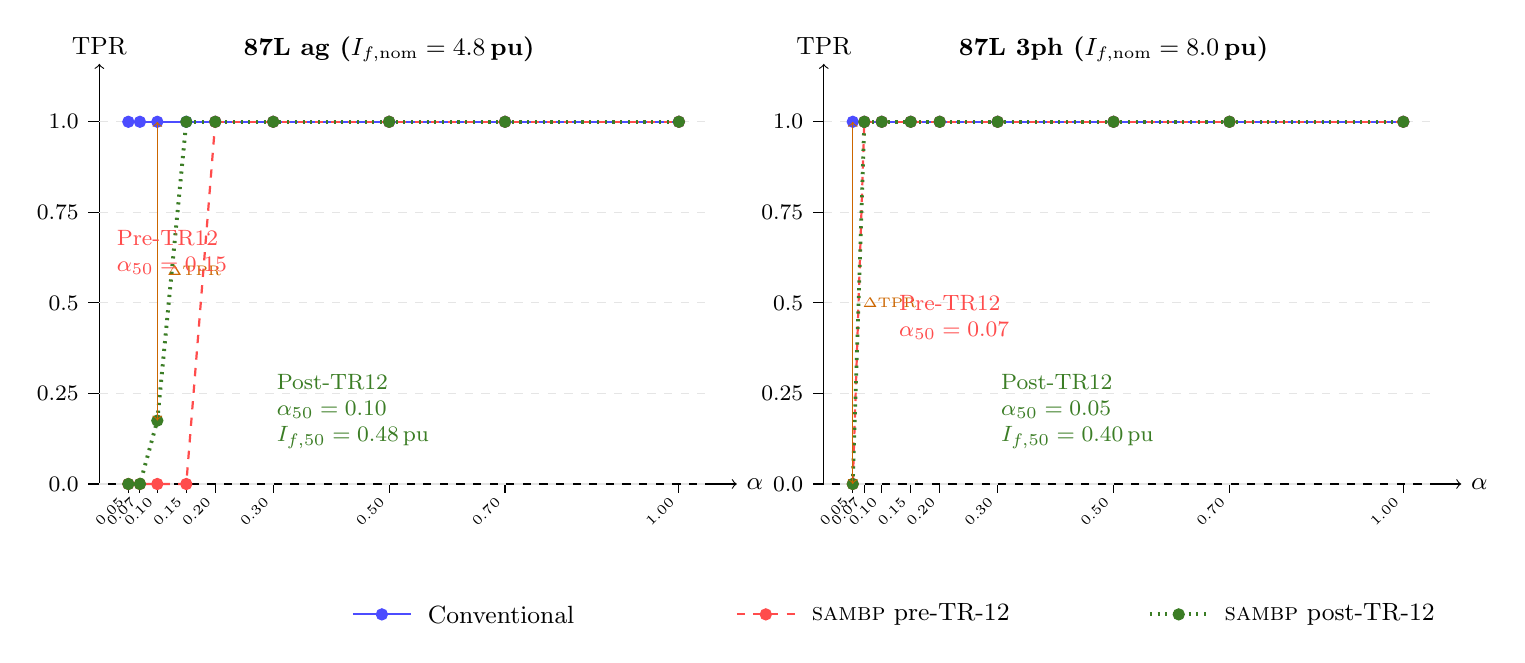
\begin{tikzpicture}[scale=0.92]

%-------------------------------------------------------------------
% Left sub-plot: ag fault  (I_f_nom = 4.8 pu)
\begin{scope}[xshift=0cm]

% Axes
\draw[->] (0,0)--(8.8,0) node[right,font=\small]{$\alpha$};
\draw[->] (0,0)--(0,5.8) node[above,font=\small]{TPR};

% X ticks
\foreach \a/\lbl in {8.0/1.00,5.6/0.70,4.0/0.50,2.4/0.30,1.6/0.20,1.2/0.15,0.8/0.10,0.56/0.07,0.4/0.05}{
    \draw (\a,0)--(\a,-0.12) node[below,font=\tiny,rotate=45,anchor=east]{\lbl};
}
% Y ticks + grid
\foreach \y/\v in {0/0.0,1.25/0.25,2.5/0.5,3.75/0.75,5.0/1.0}{
    \draw (0,\y)--(-0.15,\y) node[left,font=\footnotesize]{\v};
    \draw[gray!20,dashed](0,\y)--(8.4,\y);
}

% Conventional (always 1.0)
\draw[blue!70,thick]
  (0.4,5.0)--(0.56,5.0)--(0.8,5.0)--(1.2,5.0)--(1.6,5.0)
  --(2.4,5.0)--(4.0,5.0)--(5.6,5.0)--(8.0,5.0);
\foreach \x in {0.4,0.56,0.8,1.2,1.6,2.4,4.0,5.6,8.0}{
    \filldraw[blue!70] (\x,5.0) circle(2.2pt);}

% Pre-TR12 SAMBP (drops to 0 at alpha<=0.15)
\draw[red!70,thick,dashed]
  (1.6,5.0)--(2.4,5.0)--(4.0,5.0)--(5.6,5.0)--(8.0,5.0);
\draw[red!70,thick,dashed]
  (0.4,0.0)--(0.56,0.0)--(0.8,0.0)--(1.2,0.0)--(1.6,5.0);
\foreach \x/\y in {8.0/5.0,5.6/5.0,4.0/5.0,2.4/5.0,1.6/5.0,1.2/0.0,0.8/0.0,0.56/0.0,0.4/0.0}{
    \filldraw[red!70] (\x,\y) circle(2.2pt);}

% Post-TR12 SAMBP (TPR=1 down to alpha=0.15, 0.175 at alpha=0.10, 0 below)
% 0.175 * 5 = 0.875 in plot coordinates
\draw[OliveGreen,thick,dotted,line width=1.4pt]
  (1.2,5.0)--(1.6,5.0)--(2.4,5.0)--(4.0,5.0)--(5.6,5.0)--(8.0,5.0);
\draw[OliveGreen,thick,dotted,line width=1.4pt]
  (0.4,0.0)--(0.56,0.0)--(0.8,0.875)--(1.2,5.0);
\foreach \x/\y in {8.0/5.0,5.6/5.0,4.0/5.0,2.4/5.0,1.6/5.0,1.2/5.0,0.8/0.875,0.56/0.0,0.4/0.0}{
    \filldraw[OliveGreen] (\x,\y) circle(2.2pt);}

% Improvement bracket
\draw[<->,orange!80!black,thin] (0.8,0.875)--(0.8,5.0)
  node[midway,right,font=\tiny]{$\Delta$TPR};

\node[font=\small\bfseries] at (4.0,6.0) {87L ag  ($I_{f,\mathrm{nom}}=4.8$\,pu)};
\node[font=\footnotesize,align=left,text=OliveGreen] at (3.5,1.0)
  {Post-TR12\\$\alpha_{50}=0.10$\\$I_{f,50}=0.48$\,pu};
\node[font=\footnotesize,align=left,text=red!70] at (1.0,3.2)
  {Pre-TR12\\$\alpha_{50}=0.15$};

\end{scope}

%-------------------------------------------------------------------
% Right sub-plot: 3ph fault  (I_f_nom = 8.0 pu)
\begin{scope}[xshift=10cm]

\draw[->] (0,0)--(8.8,0) node[right,font=\small]{$\alpha$};
\draw[->] (0,0)--(0,5.8) node[above,font=\small]{TPR};

\foreach \a/\lbl in {8.0/1.00,5.6/0.70,4.0/0.50,2.4/0.30,1.6/0.20,1.2/0.15,0.8/0.10,0.56/0.07,0.4/0.05}{
    \draw (\a,0)--(\a,-0.12) node[below,font=\tiny,rotate=45,anchor=east]{\lbl};
}
\foreach \y/\v in {0/0.0,1.25/0.25,2.5/0.5,3.75/0.75,5.0/1.0}{
    \draw (0,\y)--(-0.15,\y) node[left,font=\footnotesize]{\v};
    \draw[gray!20,dashed](0,\y)--(8.4,\y);
}

% Conventional
\draw[blue!70,thick]
  (0.4,5.0)--(0.56,5.0)--(0.8,5.0)--(1.2,5.0)--(1.6,5.0)
  --(2.4,5.0)--(4.0,5.0)--(5.6,5.0)--(8.0,5.0);
\foreach \x in {0.4,0.56,0.8,1.2,1.6,2.4,4.0,5.6,8.0}{
    \filldraw[blue!70] (\x,5.0) circle(2.2pt);}

% Pre-TR12 SAMBP (drops to 0 at alpha<=0.07)
\draw[red!70,thick,dashed]
  (0.56,5.0)--(0.8,5.0)--(1.2,5.0)--(1.6,5.0)
  --(2.4,5.0)--(4.0,5.0)--(5.6,5.0)--(8.0,5.0);
\draw[red!70,thick,dashed]
  (0.4,0.0)--(0.56,5.0);
\foreach \x/\y in {8.0/5.0,5.6/5.0,4.0/5.0,2.4/5.0,1.6/5.0,1.2/5.0,0.8/5.0,0.56/5.0,0.4/0.0}{
    \filldraw[red!70] (\x,\y) circle(2.2pt);}

% Post-TR12 SAMBP (TPR=1 down to alpha=0.07, 0 at alpha=0.05)
\draw[OliveGreen,thick,dotted,line width=1.4pt]
  (0.56,5.0)--(0.8,5.0)--(1.2,5.0)--(1.6,5.0)
  --(2.4,5.0)--(4.0,5.0)--(5.6,5.0)--(8.0,5.0);
\draw[OliveGreen,thick,dotted,line width=1.4pt]
  (0.4,0.0)--(0.56,5.0);
\foreach \x/\y in {8.0/5.0,5.6/5.0,4.0/5.0,2.4/5.0,1.6/5.0,1.2/5.0,0.8/5.0,0.56/5.0,0.4/0.0}{
    \filldraw[OliveGreen] (\x,\y) circle(2.2pt);}

% Improvement bracket at alpha=0.05
\draw[<->,orange!80!black,thin] (0.4,0.0)--(0.4,5.0)
  node[midway,right,font=\tiny]{$\Delta$TPR};

\node[font=\small\bfseries] at (4.0,6.0) {87L 3ph  ($I_{f,\mathrm{nom}}=8.0$\,pu)};
\node[font=\footnotesize,align=left,text=OliveGreen] at (3.5,1.0)
  {Post-TR12\\$\alpha_{50}=0.05$\\$I_{f,50}=0.40$\,pu};
\node[font=\footnotesize,align=left,text=red!70] at (1.8,2.3)
  {Pre-TR12\\$\alpha_{50}=0.07$};

\end{scope}

%-------------------------------------------------------------------
% Shared legend
\draw[blue!70,thick] (3.5,-1.8)--(4.3,-1.8);
\filldraw[blue!70] (3.9,-1.8) circle(2.2pt);
\node[right,font=\small] at (4.4,-1.8) {Conventional};

\draw[red!70,thick,dashed] (8.8,-1.8)--(9.6,-1.8);
\filldraw[red!70] (9.2,-1.8) circle(2.2pt);
\node[right,font=\small] at (9.7,-1.8) {\textsc{sambp} pre-TR-12};

\draw[OliveGreen,thick,dotted,line width=1.4pt] (14.5,-1.8)--(15.3,-1.8);
\filldraw[OliveGreen] (14.9,-1.8) circle(2.2pt);
\node[right,font=\small] at (15.4,-1.8) {\textsc{sambp} post-TR-12};

\end{tikzpicture}
